This work uses the charge method outlined by \textcite{Furlani2001}, where a fictitious magnetic charge is distributed over the surface of each magnet, and assumes a relative permeability \(\mu_r\) of unity with constant uniform magnetisation \(\mathbf{M}\). Recent studies have detailed methods for including the effect of non-unity permeability in calculations of the magnetic field from permanent magnets \cite{Dam2016}. While out of the scope for the current work, such methods can also be applied to the results presented here.

In this method, polyhedral permanent magnets are decomposed into the polygonal facets that make up the surface of the polyhedron. Each polygonal facet has a fictitious magnetic charge distribution, which creates a magnetic field and thus induces forces and torques on other magnets.

In this work, two magnets are defined, magnet A and magnet B. The force and torque on magnet B is calculated due to the field produced by magnet A. An algorithm to analytically calculate the field due to magnet A is presented. Then, a mesh is applied to the surface of magnet B and the field due to magnet A is calculated at each mesh element. Finally, numeric integration is performed to find the force and torque on magnet B. These steps are outlined in more detail below.
\begin{figure*}
	\centering
	\begin{subfigure}{0.4\textwidth}
		\centering
		\tdplotsetmaincoords{70}{110}
		\tdplotsetrotatedcoords{0}{0}{0}
		\begin{tikzpicture}[scale = 0.45,tdplot_rotated_coords]
		
		\coordinate (p1b) at (0,1,5);
		\coordinate (p2b) at (0,3,5);
		\coordinate (p3b) at (0,6,3);
		\coordinate (p4b) at (0,6,-2);
		\coordinate (p5b) at (0,1,-2);
		\coordinate (p1f) at (5,1,5);
		\coordinate (p2f) at (5,3,5);
		\coordinate (p3f) at (5,6,3);
		\coordinate (p4f) at (5,6,-2);
		\coordinate (p5f) at (5,1,-2);
		
		\draw (p1b) -- (p2b) -- (p3b) -- (p4b);% -- (p5b) -- cycle;
		\draw[fill=black!10] (p1f) -- (p2f) -- (p3f) -- (p4f) -- (p5f) -- cycle;
		\draw (p1f) -- (p1b);
		\draw (p2f) -- (p2b);
		\draw (p3f) -- (p3b);
		\draw (p4f) -- (p4b);
		
		\draw[->,thick] (5,3.5,0.5) -- (5,3.5,2.5);
		\node (M1) at (5,4,1.5) {\textbf{M}};
		\end{tikzpicture}
		\caption{}
		\label{fig:p13dpolyhedron}
	\end{subfigure}
	
	\vspace{20pt}
	
	\begin{subfigure}{0.4\textwidth}
		\centering
		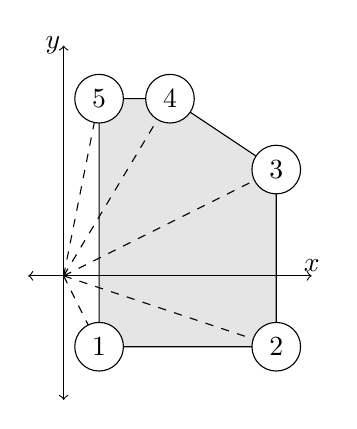
\begin{tikzpicture}[scale=0.45]
		\coordinate (origin) at (0,0);
		\coordinate (p5) at (1,5);
		\coordinate (p4) at (3,5);
		\coordinate (p3) at (6,3);
		\coordinate (p2) at (6,-2);
		\coordinate (p1) at (1,-2);
		
		\filldraw[fill = black!10] (p1) -- (p2) -- (p3) -- (p4) -- (p5) -- cycle;
		
		\draw[dashed] (origin) node {} -- (p1) node[circle,fill=white,draw,solid] {1};
		\draw[dashed] (origin) node {} -- (p2) node[circle,fill=white,draw,solid] {2};
		\draw[dashed] (origin) node {} -- (p3) node[circle,fill=white,draw,solid] {3};
		\draw[dashed] (origin) node {} -- (p4) node[circle,fill=white,draw,solid] {4};
		\draw[dashed] (origin) node {} -- (p5) node[circle,fill=white,draw,solid] {5};
		
		\node (x) at (7,0.3){\(x\)};
		\node (y) at (-0.3,6.5){\(y\)};
		
		\draw [<->] (-1,0) -- (7,0);
		\draw [<->] (0,-3.5) -- (0,6.5);
		\end{tikzpicture}
		\caption{}
		\label{fig:p1polygondecomposition}
	\end{subfigure}
	~
	\begin{subfigure}{0.4\textwidth}
		\centering
		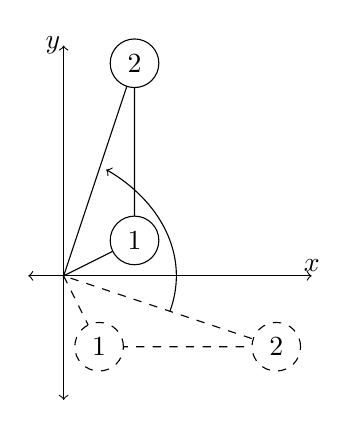
\begin{tikzpicture}[scale=0.45]
		\coordinate (origin) at (0,0);
		\coordinate (p2) at (2,1);
		\coordinate (p1) at (2,6);
		
		\draw[solid] (p1) -- (origin) -- (p2) -- cycle;
		\path (p1) node[circle,fill=white,draw,solid] {2} -- (p2) node[circle,fill=white,draw,solid] {1};
		
		\draw[dashed] (0,0) -- (1,-2) -- (6,-2) -- cycle;
		\path (6,-2) node[circle,fill=white,draw,dashed] {2} -- (1,-2) node[circle,fill=white,draw,dashed] {1};
		
		\node (x) at (7,0.3){\(x\)};
		\node (y) at (-0.3,6.5){\(y\)};
		
		\draw [<->] (-1,0) -- (7,0);
		\draw [<->] (0,-3.5) -- (0,6.5);
		
		\draw[<-] (1.2,3) to [out=-30,in=70] (3,-1.0);
		\end{tikzpicture}
		\caption{}
		\label{fig:p1makingtriangles}
	\end{subfigure}
	\caption{A simple polyhedral permanent magnet, created by chamfering one edge of a cuboid (a). The magnet is magnetised vertically upward, as indicated by the arrow. Each facet is rotated such that it is parallel to the \(XY\)-plane and a line is drawn from the \(z\)-axis to each vertex (b), creating \(n\) triangles from the \(n\)-sided facet. Each triangle is rotated such that the edge joining the two vertices is parallel to the \(y\)-axis (c). The field of each rotated triangle is calculated then rotated back to the initial state. Each of these fields is added to give the total field of the facet. This process is then repeated for all other facets of the polyhedron to give the total field of the polyhedron.}
	\label{fig:p1decomposethepolygon}
\end{figure*}

\subsection{Calculation of the field due to magnet A}
The field due to magnet A is found using a similar method to \textcite{Rubeck2013}, but the equations are more efficient. Unlike the field equations presented by \textcite{Janssen2010}, all expressions and sub-expressions here are purely real. The magnetic field is found by first taking a polyhedral permanent magnet, such as that shown in Figure \ref{fig:p13dpolyhedron}\footnote{The magnet shown in Figure \ref{fig:p1decomposethepolygon} is a 5 unit (width) by 7 unit (height) by 5 unit (depth) cuboid, with a chamfer cutting the top face to a width of 2 units and one of the vertical faces to a height of 5 units.}, and decomposing it into its polygonal facets. Each facet is rotated about the \(x\)- and \(y\)-axes, making it parallel to the \(XY\)-plane, using the rotation matrix \(R_{xy}\), given by
\begin{equation}
R_{xy} = \begin{bmatrix}
\frac{n_z}{\sqrt{n_x^2+n_z^2}} & 0 & -\frac{n_x}{\sqrt{n_x^2+n_z^2}} \\
-\frac{n_xn_y}{\sqrt{n_x^2+n_z^2}} & \sqrt{n_x^2+n_z^2} & \frac{n_yn_z}{\sqrt{n_x^2+n_z^2}} \\
n_x & n_y & n_z
\end{bmatrix} \text{,}
\end{equation}
\noindent where \(\hat{\mathbf{n}} = \left[ n_x, n_y, n_z \right]\) is the outward-facing unit normal vector of each facet. Once parallel to the \(XY\)-plane, a line is drawn from the \(z\)-axis to each polygon vertex, as shown in Figure \ref{fig:p1polygondecomposition}, forming \(n\) triangles, where \(n\) is the number of sides of the polygon. It is important that the last triangle is defined from vertex \(n\) to vertex 1. This is because this algorithm calculates the field due to each triangle, which may include area not covered by the polygon. For example, the triangle between the \(z\)-axis, vertex 1, and vertex 5 of the polygon shown in Figure \ref{fig:p1polygondecomposition} is not part of the polygon, but the field of it is calculated from the first four triangles. The fifth triangle is defined from vertex 5 to vertex 1, effectively creating a triangle which subtracts the field due to this area outside the polygon.

After \(n\) triangles have been defined, each one is rotated so that the side joining the two vertices is parallel to the \(y\)-axis, shown in Figure \ref{fig:p1makingtriangles}. This is done using the rotation matrix
\begin{equation}
R_z = \begin{bmatrix}
-\frac{y_2-y_1}{\sqrt{\left( y_2-y_1 \right)^2 + \left( x_2-x_1 \right)^2}} & \frac{x_2-x_1}{\sqrt{\left( y_2-y_1 \right)^2 + \left( x_2-x_1 \right)^2}} & 0 \\
-\frac{x_2-x_1}{\sqrt{\left( y_2-y_1 \right)^2 + \left( x_2-x_1 \right)^2}} & -\frac{y_2-y_1}{\sqrt{\left( y_2-y_1 \right)^2 + \left( x_2-x_1 \right)^2}} & 0 \\
0 & 0 & 1
\end{bmatrix} \text{,}\\
\end{equation}
\noindent where \(x_1\), \(x_2\), \(y_1\), and \(y_2\) are the \(x\) and \(y\) coordinates of the two vertices not intersecting the \(z\)-axis before the triangle is rotated.

After rotation, the charge model outlined by \textcite{Furlani2001} can be used to solve for the magnetic field due to each triangle using the following expression.
\begin{eqnarray}\label{eqn:p1chargeB}
\mathbf{B} = -\frac{\mu_0}{4\pi} \int_{V} \left( \nabla \cdot \mathbf{M} \right) \frac{\mathbf{x} - \mathbf{x}'}{\left| \mathbf{x} - \mathbf{x}' \right|^3} \ dv' + \frac{\mu_0}{4\pi} \oint_{S} \left( \mathbf{M} \cdot \hat{\mathbf{n}} \right) \frac{\mathbf{x} - \mathbf{x}'}{\left| \mathbf{x} - \mathbf{x}' \right|^3} \ ds' \text{,}
\end{eqnarray}
\noindent where \(\mathbf{B}\) is the magnetic field, \(\mu_0\) is the magnetic permeability of free space, \(\mathbf{M}\) is the magnetisation vector, \(\mathbf{x}\) is the point of interest, \(\mathbf{x}'\) is a point on or inside the magnet, \(d{\mathrm{v}}'\) is a volume element of the magnet, and \(d{\mathrm{s}}'\) is a surface element of the magnet.

Assuming constant uniform magnetisation \(\mathbf{M}\), the first integral in Equation (\ref{eqn:p1chargeB}) disappears as \(\nabla \cdot \mathbf{M}=0\). The magnetic field due to each triangle can then be found by solving the second integral, giving
\begin{align}\label{eqn:p1trieqns}
    B_{x\Delta} &= \frac{\mu_0 \mathbf{M} \cdot \mathbf{\hat{n}}}{4\pi} \left( \frac{1}{2}\log\frac{\left( l_{az2}+y_2\right)\left(l_{az1}-y_1\right)}{\left(l_{az2}-y_2\right)\left(l_{az1}+y_1\right)} + \right. \nonumber \\
	& \quad \quad \quad \quad \quad \quad \quad \left. \frac{y_1}{2l_{a1}} \log \frac{l_{az1}+l_{a1}}{l_{az1}-l_{a1}} - \frac{y_2}{2l_{a2}} \log \frac{l_{az2}+l_{a2}}{l_{az2}-l_{a2}} \right) \nonumber \\
    & \quad \nonumber \\
	B_{y\Delta} &= \frac{\mu_0 \mathbf{M} \cdot \mathbf{\hat{n}}}{4\pi} \left( \frac{a}{2l_{a2}} \log \frac{l_{az2}+l_{a2}}{l_{az2}-l_{a2}} - \frac{a}{2l_{a1}} \log \frac{l_{az1}+l_{a1}}{l_{az1}-l_{a1}} \right) \\
    & \quad \nonumber \\
	B_{z\Delta} &= -\frac{\mu_0 \mathbf{M} \cdot \mathbf{\hat{n}}}{4\pi} \left( \text{sgn} \left( z' \right) \arctan \frac{ay_2-ay_1}{y_1y_2+a^2} + \right. \nonumber \\
	& \quad \quad \quad \quad \quad \quad \quad \left. \arctan \frac{az'y_1l_{az2}-az'y_2l_{az1}}{z'^2y_1y_2+a^2l_{az1}l_{az2}} \right)  \text{,} \nonumber
\end{align}
%\begin{subequations}
%	\begin{eqnarray}
%	B_{x\Delta} &=& \frac{\mu_0 \mathbf{M} \cdot \mathbf{\hat{n}}}{4\pi} \left( \frac{1}{2}\log\frac{\left( l_{az2}+y_2\right)\left(l_{az1}-y_1\right)}{\left(l_{az2}-y_2\right)\left(l_{az1}+y_1\right)} + \right. \nonumber \\
%	& & \left. \frac{y_1}{2l_{a1}} \log \frac{l_{az1}+l_{a1}}{l_{az1}-l_{a1}} - \frac{y_2}{2l_{a2}} \log \frac{l_{az2}+l_{a2}}{l_{az2}-l_{a2}} \right) \\
%	&&\nonumber\\
%	B_{y\Delta} &=& \frac{\mu_0 \mathbf{M} \cdot \mathbf{\hat{n}}}{4\pi} \left( \frac{a}{2l_{a2}} \log \frac{l_{az2}+l_{a2}}{l_{az2}-l_{a2}} - \right. \nonumber \\
%	& & \left. \frac{a}{2l_{a1}} \log \frac{l_{az1}+l_{a1}}{l_{az1}-l_{a1}} \right)  \\
%	&&\nonumber\\
%	B_{z\Delta} &=& -\frac{\mu_0 \mathbf{M} \cdot \mathbf{\hat{n}}}{4\pi} \left( \text{sgn} \left( z' \right) \arctan \frac{ay_2-ay_1}{y_1y_2+a^2} + \right. \nonumber \\
%	& & \left. \arctan \frac{az'y_1l_{az2}-az'y_2l_{az1}}{z'^2y_1y_2+a^2l_{az1}l_{az2}} \right)  \text{,}
%	\end{eqnarray}
%\end{subequations}
\noindent with
\begin{align*}
l_{a1} &= \sqrt{a^2+y_1^2} \nonumber \\
l_{a2} &= \sqrt{a^2+y_2^2} \nonumber \\
l_{az1} &= \sqrt{a^2+y_1^2+z'^2} \nonumber \\
l_{az2} &= \sqrt{a^2+y_2^2+z'^2} \nonumber \text{,}
\end{align*}
\noindent where \(\log()\) is the natural logarithm, \(\text{sgn}()\) is the sign function, \(\arctan()\) is the arctangent, and \(\left( 0,0,z' \right)\), \(\left( a,y_1,z' \right)\), and \(\left( a,y_2,z' \right)\) are the coordinates of the triangle vertices after rotation. This field can then be rotated back to the original position using the rotation matrix \(R_z^{-1}\). The field due to each triangle is summed, giving the field of the polygonal facet. Then, the field due to the polygonal facet is rotated back to the original position using the rotation matrix \(R_{xy}^{-1}\). The total field due to magnet A is then calculated by summing the field contribution of each polygonal facet. This field calculation gives the magnetic field at the origin, but the magnetic field at any point can be calculated using a coordinate translation such that the point of interest lies on the origin. The magnetic field calculation can be represented using Algorithm \ref{alg:p1alg1}.
\begin{algorithm}
	\caption{Calculate the magnetic field of a polyhedral permanent magnet}
	\begin{algorithmic}[1]
		\State Set \(\mathbf{B} = [0,0,0]^\textsf{T}\).
		\For {each \(n\)-sided facet of the polyhedron}
		\State \parbox[t]{\dimexpr\linewidth-\leftmargin-\labelsep-\labelwidth}{Define the vertices in an anticlockwise order when looking at the polyhedron from the outside.}\newline
		\State \parbox[t]{\dimexpr\linewidth-\leftmargin-\labelsep-\labelwidth}{Store these in a \(3\times n\) matrix \(P\) such that each column represents a vertex.}\newline
		\State \parbox[t]{\dimexpr\linewidth-\leftmargin-\labelsep-\labelwidth}{Copy the first column of \(P\) and add it as the \(\left(n+1\right)\)th column.}\newline
		\State \parbox[t]{\dimexpr\linewidth-\leftmargin-\labelsep-\labelwidth}{Evaluate the matrix \(R_{xy}\) and create a new matrix \(P_{xy}\) given by \(P_{xy} = R_{xy}P\).}\newline
		\For {\(j=1,\dots,n\)}
		\State \parbox[t]{\dimexpr\linewidth-\leftmargin-\labelsep-\labelwidth}{Using the \(j\)th and \(\left(j+1\right)\)th columns of \(P_{xy}\), calculate \(R_z\). Create \(P_z\) given by \(P_z = R_zP_{xy}\).}\newline
		\State \parbox[t]{\dimexpr\linewidth-\leftmargin-\labelsep-\labelwidth}{Evaluate \(\textbf{B}_\Delta\) using the points from \(P_z\) and Equation (\ref{eqn:p1trieqns}).}\newline
		\State \label{alg:p1enum2}Add the value of \(\left(R_{xy}^{-1}R_z^{-1}\textbf{B}_\Delta\right)\) to \(\mathbf{B}\).
		\EndFor
		\EndFor
		\State The field at the origin is now equal to \(\mathbf{B}\).
	\end{algorithmic}\label{alg:p1alg1}
\end{algorithm}

Algorithm \ref{alg:p1alg1} was implemented on the three-dimensional polyhedral magnet shown in Figure \ref{fig:p1decomposethepolygon}. Flux lines were drawn on the plane of symmetry to give a visual representation of the magnetic field, and are shown in Figure \ref{fig:p1fluxlines}.
\begin{figure}
	\centering
	\includegraphics[trim = 3cm 10cm 3cm 10cm,width=0.8\linewidth]{p1/p1FIG2}
	\caption{The magnetic flux lines of the polyhedral magnet shown in Figure \ref{fig:p1decomposethepolygon}. The flux lines travel from the north pole (top) of the magnet to the south pole (bottom) of the magnet. The flux lines behave similarly to that of a cuboidal magnet in most regions due to the magnet being almost cuboidal. However, in the top right region, the flux lines differ from those of a cuboidal magnet due to the chamfer.}
	\label{fig:p1fluxlines}
\end{figure}

\subsection{Force and torque on magnet B}
The force and torque on magnet B is found using numeric integration of the magnetic field due to magnet A over the surface of magnet B, as described by \textcite{Furlani2001}. This is done by numerically solving the integrals
\begin{subequations}
    \begin{eqnarray}
	\mathbf{F}_\text{B} &=& \oint_{S_\text{B}} \left( \mathbf{M}_\text{B} \cdot \mathbf{\hat{n}}_\text{B} \right) \mathbf{B}_\text{A}\  ds_\text{B} \text{,} \\
	\mathbf{T}_\text{B} &=& \oint_{S_\text{B}} \left( \mathbf{M}_\text{B} \cdot \mathbf{\hat{n}}_\text{B} \right) \left( \mathbf{r}_\text{B} \times \mathbf{B}_\text{A} \right)\ ds_\text{B} \text{,}
	\end{eqnarray}
\end{subequations}
\noindent where \({S_\mathrm{B}}\) is the surface of magnet B, \({\mathbf{M}_\mathrm{B}}\) is the magnetisation vector of magnet B, \({\mathbf{\hat{n}}_\mathrm{B}}\) is the outward-facing normal vector of the surface of magnet B, \({\mathbf{B}_\mathrm{A}}\) is the field due to magnet A, and \({\mathbf{r}_\mathrm{B}}\) is the vector from the point of rotation of magnet B to the surface of magnet B.

To solve these expressions, a mesh is defined on the surface of magnet B. This mesh must be defined such that the field due to magnet A is relatively constant over each element. The field due to magnet A is evaluated at the centre of each mesh element using Algorithm \ref{alg:p1alg1}. The force and torque on magnet B can be found by numerically integrating the field at each element with area \(A_i\), as shown in Equation (\ref{eqn:p1numericforcetorque}), where \(\mathbf{b}_i\) is the field due to magnet A at the centre of each mesh element.
\begin{subequations}
	\label{eqn:p1numericforcetorque}
	\begin{eqnarray}
	\mathbf{F}_\text{B} &=& \sum_i \left( \mathbf{M}_\text{B} \cdot \mathbf{\hat{n}}_\text{B} \right) {\mathbf{b}_i A_i} \text{,} \\
	\mathbf{T}_\text{B} &=& \sum_i \left( \mathbf{M}_\text{B} \cdot \mathbf{\hat{n}}_\text{B} \right) \left( {\mathbf{r}_i \times \mathbf{b}_i} \right) A_i \text{.}
	\end{eqnarray}
\end{subequations}

This process can be represented programmatically using Algorithm \ref{alg:p1alg2}.
\begin{algorithm}
	\caption{Calculate the force and torque on a polyhedral permanent magnet}
	\begin{algorithmic}[1]
		\State Apply a mesh to the surface of magnet B.
		\For {each mesh element \(i\) on the surface of magnet B}
		\State \parbox[t]{\dimexpr\linewidth-\leftmargin-\labelsep-\labelwidth}{Translate the entire system so the centre of the element lies on the origin.}\newline
		\State \parbox[t]{\dimexpr\linewidth-\leftmargin-\labelsep-\labelwidth}{Calculate the magnetic field strength from magnet A using Algorithm \ref{alg:p1alg1}.}\newline
		\State \parbox[t]{\dimexpr\linewidth-\leftmargin-\labelsep-\labelwidth}{Calculate the cross product of the torque moment arm and the magnetic field strength \(\mathbf{r}\times\mathbf{b}\).}\newline
		\State Calculate the quantity \(\mathbf{M}\cdot\hat{\mathbf{n}}\) for the element.
		\State \parbox[t]{\dimexpr\linewidth-\leftmargin-\labelsep-\labelwidth+4mm}{Set \(\mathbf{f}_i=\left(\mathbf{M}\cdot\hat{\mathbf{n}}\right)\mathbf{b}A_i\) and \(\mathbf{\tau}_i=\left(\mathbf{M}\cdot\hat{\mathbf{n}}\right)\left(\mathbf{r}\times\mathbf{b}\right)A_i\) where \(A_i\) is the area of the element.}\newline
		\EndFor
		\State {Set \(\mathbf{F} = \sum_i\mathbf{f}_i\) and \(\mathbf{T} = \sum_i\mathbf{\tau}_i\).}
		\State The force and torque on magnet B are given by \(\mathbf{F}\) and \(\mathbf{T}\) respectively.
	\end{algorithmic}\label{alg:p1alg2}
\end{algorithm}

Thus the exact magnetic field due to a polyhedral permanent magnet has been analytically calculated, and the force and torque on a second polyhedral magnet has been numerically calculated using the analytic field solution.